\section{Sensibility Testbed Architecture}\label{sec-design}

\begin{figure}
\center{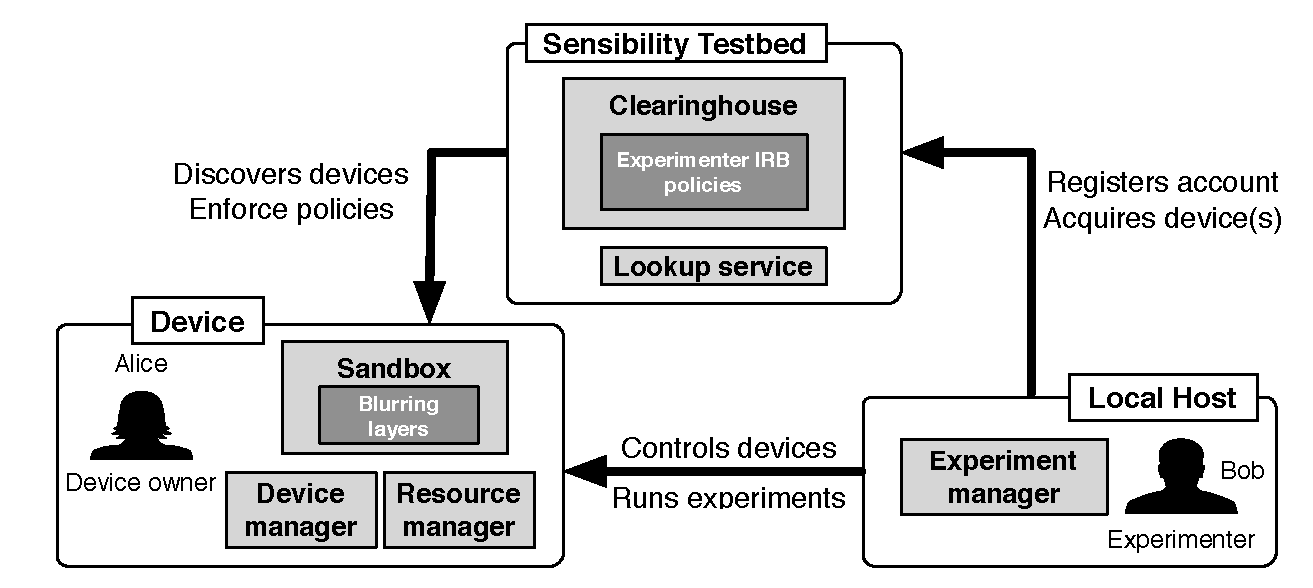
\includegraphics[width=\columnwidth]{figs/arch.pdf}}
%\vspace*{-20pt}
\caption{\small Sensibility Testbed architecture. \label{fig-arch}}
\end{figure}

The Sensibility Testbed architecture's three main components are critical 
to its operation. In this section, we discuss each of these components in 
greater detail, describing their functions and introducing several key 
techniques that make the testbed's enhanced security possible. 

\subsection{Device Software}\label{sec-repy}

%In Sensibility Testbed, all experiments execute in a secure 
%sandbox on the end devices.
%Experimenters' code executes in a sandbox that isolates the 
%experiment code from the device host system. 
The device software of Sensibility Testbed is the only one of the three 
components that runs on end users' devices. It is divided into three 
parts: a secure sandbox called Repy (Restricted Python), a resource 
manager that facilitates the interaction between researchers and the 
sandbox, and a device manager that allows the device owner to control 
if the sandbox and resource manager can run on the device.
The Repy sandbox is the most important in the device software. This 
security-reviewed sandbox~\cite{cappos2010retaining} mitigates the 
impact of bugs in experimenter code by providing security isolation 
and performance isolation\footnote{\scriptsize 
This sandbox has been used successfully for more than six years in our 
prior work, the Seattle testbed~\cite{seattle}.}. 
%Instead of developing full-fledged Android apps, all 
%experiments in Sensibility Testbed are written in a language
%similar to Python, and run in a secure %Python-based
Researchers use a Python-like programming interface~\cite{repyv2}
to write experiment code, upload the code and execute it in the
sandbox on remote devices. The programming interface includes functions for networking, 
file system access, threading, locking, logging, and so on. To access sensors, 
the sandbox also has a set of sensor functions~\cite{sensors}. 
%Details about implementing the Repy sandbox for mobile 
%devices are described in Section~\ref{sec-repy-ext}.
%
%However, the current Repy sandbox does not include calls to access sensors. 
%%To obtain the sensor data, we need to extend the sandbox. 
%The extended Repy sandbox that allows sensor access  
%will be described in Section~\ref{sec-repy-ext}.
Another important feature of the Repy sandbox allows us to change the 
behavior of its programming interface, and control the 
data gathered from the device to adapt to any IRB proscribed limits. 
%For  an experiment
%that involves GPS location, a privacy policy might restrict the
%level of data granularity available to the experiment. For example, it can
%obfuscate GPS location such that it only identifies the center
%of the city that the device is located in, rather than the exact
%location. Using the same technique, 
For example, the sandbox can anonymize the IP address of a device, constrain  
the frequency of access to GPS locations, and disable
access to cameras. 
%Such privacy protection is a contribution of Sensibility Testbed, 
%which does not exist in any prior work. 
The details of policy implementation are presented in 
Section~\ref{sec-layer} and \ref{sec-nanny}.

The second part of the device software, called a resource manager, 
establishes a trust relationship between a device and a researcher. It 
manages a researcher's access to the sandboxes on a device, and
controls the start and stop of the sandboxes on the device. The 
resource manager controls which researchers can access the 
sandbox on any given device, and communicates with the clearinghouse
or experiment manager. If multiple researchers have access to 
the same device, the resource manager splits the resources in the 
sandbox among the researchers, and partitions the one sandbox 
into several smaller ones. In order for the clearinghouse or a 
researcher's experiment manager to discover the sandbox on a 
device, the resource manager also contacts a lookup service that 
announces the existence of the available devices. An example is 
given in Section~\ref{sec-ops}.

The last part of the device software is a device manager that 
allows device owners to manage the software running on their 
devices. This is the only part of device software that a device owner 
will interact with directly. With the device manager, a device owner  
can install and remove the device software, and start and stop the 
operations. The device manager also provides a user interface to 
allow a device owner to opt out of any experiment. Thus, the device 
owner has the freedom to choose what experiments will be allowed 
to run on the phone or tablet.


\subsection{Clearinghouse}\label{sec-ch}
The clearinghouse~\cite{ch} is a testbed server that has two 
responsibilities. First, it keeps track of devices and grants 
researchers access to available devices; and second, it
sets up the relevant IRB policies for each individual experiment that 
must be enforced through the sandboxes on remote devices.
%It allows experimenters to register accounts and share 
%access to a common pool of devices.
Researchers register their experiments at the clearinghouse, and 
provide their institution's IRB 
policies. When an account is approved, the researcher is assigned 
a pair of public/private \textit{authentication keys} by the 
clearinghouse, to authenticate himself with the clearinghouse. This
researcher can then sign into his account and request a 
number of sandboxes for his experiment. The clearinghouse 
looks up available sandboxes on behalf of the researcher by 
querying the lookup service. Once a sandbox is discovered, the 
clearinghouse stores the sandbox's meta information, 
%\textit{identification key}, 
and assigns it to the researcher's experiment account. 

Besides assigning devices, the clearinghouse also has the role of 
instructing the sandboxes assigned to this researcher to add the IRB 
policies specified during registration. The clearinghouse does so 
by communicating with the resource managers on those devices, which 
control the code executed in the sandboxes. The involvement of the 
clearinghouse in any given experiment ends 
after the researcher deploys his code to the devices. It does not store any
data on the researcher's behalf. 
This Sensibility Testbed clearinghouse 
protocol for research with device owners has been approved by
the IRB at New York University (IRB \# 15-10751). An example 
of this protocol in operation is also given in Section~\ref{sec-ops}.

%However, it can direct the release of data to a server designated by the 
%researcher. To do so, the experimenter must register
%his server by providing its certificate and URL to the
%clearinghouse, which will then instruct the devices
%accessible to the experimenter that all the sensor data collected should be
%sent to this server. The sandboxes on these devices will issue
%\texttt{HTTPS POST} using the server's certificate, and send encrypted
%data to the experimenter's server.

%The key role of this component is to facilitate device sharing, 
%which relieves individual experimenters from repeatedly 
%recruiting devices for each experiment.
%
%Note that in Sensibility Testbed, there are two types of keys. A device
%owner has an \textit{identification key} to identify the app installed on a 
%device. This key is mostly used by a lookup service. 

%This pair of keys are mostly used by the clearinghouse and 
%experiment manager.

%\lois{have you introduced the idea of keys yet? If not, I think this needs to be explained.}


\subsection{Experiment Manager}\label{sec-emt}

The last component in the testbed is an experiment manager, which a 
researcher can download to his own computer and use to run code through 
%which contains Bob's private key, \path{key.bob-priv}, 
the sandboxes on the remote devices. 
The researcher uses the experiment manager as a light-weight command line 
console~\cite{demo-kit} to directly access the remote devices, upload 
experiment code written in the Repy programming interface, and
communicate with the resource manager on the device to start 
or stop the execution of the experiment. To authenticate himself with 
the remote sandbox, the researcher uses 
his public/private key pairs to establish a secure connection from his
computer. The experiment manager can also be used to download data 
from the remote devices to the researcher's local computer, or
the researcher can set up his own server to store the data\footnote{\scriptsize
If an experimenter stores data on his own server, he must use protective
measures to ensure that data sent from the mobile devices is
properly encrypted, and the server storage cannot be tampered
with by any other parties. This is enforced by requiring the experimenter to register
his server by providing its certificate and URL to our
clearinghouse. Following receipt of this data, the clearinghouse will instruct the devices
accessible to the experimenter that all the sensor data collected should be
sent to this server. The sandboxes on these devices will issue
\texttt{HTTPS POST} using the server's certificate, and send encrypted
data to the experimenter's server.}. 
If an experimenter stores data on his own server, he must use protective
measures to ensure that data sent from the mobile devices is
properly encrypted, and the server storage cannot be tampered
with by any other parties. Researchers can also opt to use a data 
store service we provide (a service called Sensevis~\cite{sensevis}, 
not shown in Figure~\ref{fig-arch}). After the data is collected, the method of 
securely storing the data will be mandated by the researcher's IRB.

\smallskip
This Sensibility Testbed clearinghouse protocol for research plays a central role in
easing the process of device recruitment and experiment setup for experimenters, 
and ensures the enforcement of privacy policies. 
%Prior to running an experiment on Sensibility Testbed, a
%experimenter first fills out a form in plain text to describe the
%purpose of the research experiment. This experiment description
%is created at the Sensibility Testbed clearinghouse
%where the researcher indicates the type of data to be collected,
%how that data will be used and stored, and so on. 
%
%Once this information is collected from the researcher, the
%clearinghouse automatically generates a set of blurring layers
%that implements the experiment policy (Section~\ref{sec-policy}). In
%Sensibility Testbed, researchers can collect data from the
%sensors on the device, such as GPS, Bluetooth, battery
%information, accelerometer, light, and orientation,
%etc. The blurring layers we provide consist of
%data access restrictions, created in accordance with
%researcher's experiment description, by using the Sensibility
%Testbed's sandboxing technique 
%(Section~\ref{sec-repy})~\cite{cappos2010retaining}. These restrictions ensure that
%the researcher cannot conduct experiments to access data that
%extend beyond the experiment policy. 
%
%This Sensibility Testbed
%clearinghouse protocol for research plays a central role in
%easing the approval process of IRB, and ensures the enforcement
%of privacy policy\footnote{The Sensibility Testbed Clearinghouse
%protocol for research with human subjects has been approved by
%the IRB at New York University. \yanyan{might need a link to
%your approval letter or ref number}}. 
Using Sensibility Testbed, device owners' privacy is protected
from any inadvertent or malicious attempt, and researchers 
are able to go through a streamlined process of device 
recruitment and experiment setup.

